\section{連続微分可能関数と常微分方程式}
\label{section:differentiable}

基本的な証明の流れは河村によるものと等しい \cite{Kawamura2010lipschitz}
まず補題 \ref{WeakFeedback} により任意の言語
$L \in \classPSPACE$ を認識する関数族$(G_u)_u, (H_u)_u$ を得る.
そして 補題\ref{DifferentiableFamily} では $(G_u)_u, (H_u)_u$ を模倣する
実関数族 $(g_u)_u, (h_u)_u$ を構成し,
それらから定理 \ref{DifferentiableIsPspace} で求める $g, h$を構成する.



\subsection{差分方程式}
\label{section:divp}

定理 \ref{DifferentiableIsPspace} と定理 \ref{KTimesIsCH} の証明では,
まず滑らかな実関数の常微分方程式によって
ある種の「離散版」常微分方程式を模倣できることを示し, 
その離散版の方程式が$\classPSPACE$困難ないし$\classCH$困難であることを示す.
この節ではその離散版の方程式である「差分方程式」を定義する.

$[n] = \{0, \dots , n-1\}$ と表記する.
関数 $G \colon [P] \times [Q] \times [R] \to \{-1, 0, 1\}$ に対して,
関数 $H \colon [P + 1] \times [Q+1] \to [R]$ が
任意の $i \in [P],\ T \in [Q]$ について以下を満たすとき,
$H$ を $G$ の \emph{差分方程式} の解と呼ぶ.
\begin{gather}
   H(i, 0) = H(0, T) = 0 
\\
   H(i + 1, T + 1) = H(i+1, T) + G(i, T, H(i, T))  \label{eq:divp}
\end{gather}
$P, Q, R$ をそれぞれ\emph{段数}, \emph{列数}, \emph{欄の大きさ}と呼ぶ.
$G$ と $H$ が常微分方程式の $g$ と $h$ に対応し,
$H(i, 0) = 0$ が $h(0) = 0$ に,
式 (\ref{eq:divp}) と同値である式 $H(i + 1, T + 1) - H(i+1, T) = G(i, T, H(i, T))$
が $h'(t) = g(t, h(t))$ と対応する.

以下では文字列 $u$ ごとに差分方程式 $G _u$ を一つ定めた族 $(G _u) _u$ を考える. 
各 $u$ に対して $G_u$ の段数と列数, 解をそれぞれ $P_u, Q_u, H_u$ としたとき,
言語 $L$ がこの族 $(G_u)_u$ によって認識されるとは,
$H_u(P_u, Q_u) = L(u)$ を満たすこととする(表 \ref{fig:divp}).
ここで言語 $L \subseteq \{0, 1\} ^*$ は
関数 $L \colon \{0, 1\} ^* \to \{0, 1\}$ と同一視し, 
$u \in L$ のとき $L (u) = 1$ としている. 

 \begin{figure}
  \label{fig:divp}
  \begin{center}
   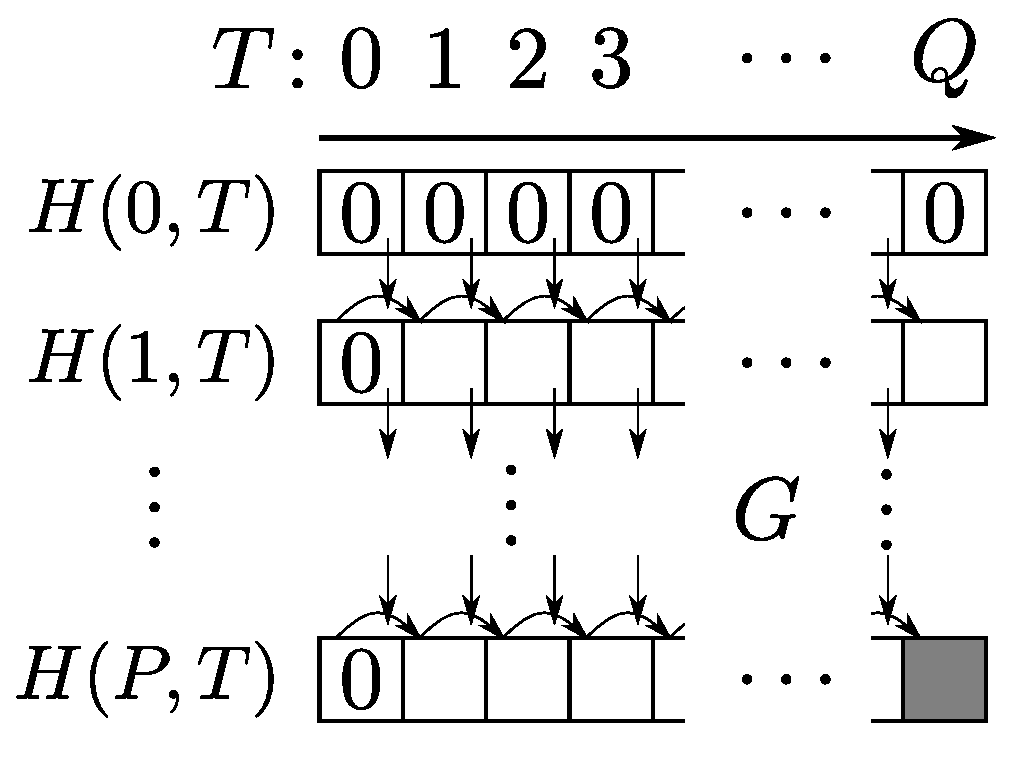
\includegraphics[height=0.2\textheight]{image/divp.eps}
  \end{center}
  \caption{差分方程式と認識される言語}
 \end{figure}

$(G_u)_u$ が{\bf 一様}であるとは,
各 $u$ について $G _u$ の段数, 列数及び欄の大きさが $|u|$ の多項式の指数($2^{\mathrm{poly} (|u|)}$)で抑えられ, 
かつ与えられた $(u, i, T, Y)$ から多項式時間で $G_u(i, T, Y)$ が
計算できることと定義する.

$G_u$ の段数がさらに $|u|$ の多項式, 対数で抑えられるとき, 
族 $(G_u) _u$ はそれぞれ\emph{多項式段}, \emph{対数段}であるという. 
多項式段, 対数段の一様関数族によって認識される言語のクラスを
それぞれ $\DIVPpoly$, $\DIVPlog$ と名づける.
この記法を使うと
河村の論文では次が示されている.

 \begin{lemma}[補題 4.7 \cite{kawamura2010lipschitz}]
  \label{WeakFeedback}
  任意の言語 $L \in \classPSPACE$ に対して,
  その言語を認識する多項式段の一様な関数族 $(G_u)_u$ が存在する.
 \end{lemma}


証明の概略を示す.
$\classPSPACE$ 完全な言語である
\textsf{QBF} を認識する $(G_u)_u$ を構成することにより,
任意の $L \in \classPSPACE$ を認識する多項式段一様な関数族 $(G_u)_u$ が存在することを示す.
ここで \textsf{QBF} とは,
文字列 $u$ を $\psi = Q_1 x_1 \cdots Q_n x_n \phi(x_1, \dots, x_n)$ と解釈したとき 
$u \in \textsf{QBF} \leftrightarrow \psi = T$ によって定義される言語である. 
ただし$Q_i$ は$\exists$ または $\forall$,  
$\phi(x_1, \dots, x_n)$ は $x_i$ 以外の変数を含まない論理式とする. 

論理式 $\psi = Q_1 x_1 \cdots Q_n x_n \phi(x_1, \dots, x_n)$ の値を
$\vee, \wedge$によってラベル付された二分木によって計算することを考える. 
量化子$Q_1 x_1$ を除き $x_1$ を $T$ と $F$ に置き換えた式をそれぞれ
$\psi_T = Q_2 x_2 \cdots Q_n x_n \phi(T, x_2, \dots, x_n)$,
$\psi_F = Q_2 x_2 \cdots Q_n x_n \phi(F, x_2, \dots, x_n)$ と置くと
$Q_1=\forall$ ならば $\psi = \psi_T \wedge \psi_F$, 
$Q_1=\exists$ ならば $\psi = \psi_T \vee \psi_F$.
つまり変数の1つ少ない2つの論理式と量化子によってもとの論理式の値も決まる.
これを再帰的に繰り返すことで $\psi$ は計算可能であり, 
それは深さ $n$ の二分木を葉から根へ値を定めていくことと等しい.
この過程は二分木の深さが段数に, 幅が列数に対応する形で
多項式段一様な関数による差分方程式で模倣可能であるため,
\textsf{QBF} を認識する多項式段一様関数族が存在する.



\subsection{$\classCH$ 困難な言語}

Wagner によって $\classCH$ の各階層 $\C_n \classP$ に対してそれぞれ完全問題が存在することが示されている\cite{wagner1986complexity}.
量化子 $\C$ を自然数 $m$, 論理式 $A(x_1, \dots, x_l)$, 
$l$ 個の論理変数の組 $\alpha$ について以下のように定義する.
\begin{equation}
 \C^m \alpha A(\alpha) 
  \longleftrightarrow 
  \Bigl|\{\alpha \in \{0,1\}^l \mid A(\alpha) = 1\}\Bigr| \ge m.
\end{equation}
$\C^1 = \exists$, $\C^{2^l} = \forall$ であり, $\C$ は $\exists, \forall$ の
一般化と言える.
言語 $\C_n B_{be}$ を以下のように定義する.
\begin{equation}
 \langle \phi(x_1, \dots, x_n), m_1, \dots, m_n \rangle \in \C_n B_{be}
 \longleftrightarrow
 \C^{m_1}{\alpha_1} \cdots \C^{m_n}{\alpha_n} \phi(\alpha_1, \dots, \alpha_n) 
\end{equation}
ただし $\langle y_1, \dots, y_i \rangle$ は組み合わせ関数,
それぞれ $x_i$, $\alpha_i$ は $l_i$ 個の論理変数の組とする.


\begin{lemma}[Theorem 7 \cite{wagner1986complexity}] \label{lemma:CnP-complete}
 $\C_n B_{be}$ は $\C_n\classP$ 完全.
\end{lemma}


各 $\C_n B_{be}$ をまとめた言語 $\C_{\log} B_{be}$ を以下のように定義する.
\[
 \langle 0^{2^n}, u \rangle \in \C_{\log} B_{be}
 \longleftrightarrow
 u \in \C_n B_{be}
\]

\begin{lemma}
 $\C_{\log} B_{be}$ は $\classCH$ 困難.
\end{lemma}

\begin{proof}
 任意の $\classCH$ の言語 $A$ はある階層 $\C_n \classP$ に属する. 
 補題 \ref{lemma:CnP-complete} より任意の $u \in \{0,1\}^*$ について
 $u \in A \leftrightarrow f(u) \in \C_n B_{be}$ 
 を満たす多項式時間関数 $f$ が存在する.
 \begin{align}
  u \in A 
  & \longleftrightarrow \langle 0^{2^n}, f(u) \rangle \in \C_{\log} B_{be}
 \end{align}
 $n$ は定数であるため $\langle 0^{2^n}, f(\cdot) \rangle$ は多項式時間関数.
 よって $A$ は $\C_n B_{be}$ に多項式時間還元可能.
\end{proof}

\begin{lemma}
 $\C_{\log} B_{be}$ を認識する対数段一様関数族 $(G_u)_u$ が存在する.
\end{lemma}

\begin{proof}
 関数族 $(G_u)_u$, $(H_u)_u$, 関数 $p$, 多項式 $q,r$ を構成する.
 $u  = \langle 0^{2^n}, 
 \langle \phi(x_1, \dots, x_n), m_1, \dots, m_n \rangle \rangle$
 と仮定する.
 
 $L = C_{\log} B_{be}$,
 $l_i = |x_i|$,
 $s_i = \sum^i_{j=1}l_j + 2i$  と表記する.
 関数 $C^m \colon \N \to \{0,1\}$ を
 \begin{equation}
  C^m(Y) 
     = \begin{cases}
       1 & (Y \ge m) \\
       0 & (Y < m) \end{cases}
 \end{equation}
 と定義する. 
 任意の $i = 0, \dots, n$ と $n-i$ 個の文字列 
 $\beta_{i+1} \in \{0,1\}^{l_{i+1}}, \dots, \beta_n \in \{0,1\}^{l_n}$ 
 について部分式
 $\C^{m_{i}}{\alpha_i} \cdots \C^{m_1}{\alpha_1}
 \phi(\alpha_1, \dots, \alpha_i, \beta_{i+1}, \dots, \beta_n)$
 の真偽値を $\phi_i(\beta_{i+1}, \dots, \beta_n)$ と表記する.
 \begin{align}
  \phi_0 &= \phi 
  \\ \label{eq:phi-step}
  \phi_{i+1}(\beta_{i+2}, \dots, \beta_n) 
  &= C^{m_{i+1}}\left(\sum\nolimits_{\alpha_i \in \{0,1\}^{l_i}} 
  \phi_i(\alpha_{i+1}, \beta_{i+2}, \dots, \beta_{n})\right) 
  \\
  \phi_n() &= L(u) 
 \end{align}
 $T \in \N$ に対し, $T_i$ を $T$ の2進表記における $i$ 桁目, 
 $T_{[i,j]} = T_{j-1} T_{j-2} \cdots T_{i+1} T_{i}$ と表記する.


 $G_u$ を $(i, T, Y) \in [n+1] \times [2^{s_n}+1] \times [2^{|u|}]$ の範囲で
 を以下のように定義する. 一段目つまり $i=0$ ならば
 \begin{equation}
  G_u(0,T,Y) = 
   (-1)^{T_{s_1}}\phi(T_{[1,s_1]}, T_{[s_1+1,s_2]},
    \dots, T_{[s_{n-1}+1,s_n]}) 
 \end{equation}
 $i \ge 1$ ならば
 \begin{equation} \label{eq:def-Gu:case0}
  G_u(i,T,Y) = 
   \begin{cases}
    (-1)^{T_{s_{i+1}}} C^{m_i}(Y) 
    & (T_{[1,s_i]} = 10 \cdots 0) \\
    0 & (\text{othewise}).
   \end{cases} 
 \end{equation}


 任意の $i \in [n+1]$, $T \in [2^{s_n}+1]$ について,
 $H_u(i,T) \in [2^{l_i}+1]$ が成りたつこと,
 および $T_{[1,s_i]} = 10 \cdots 0$ ならば
 \begin{equation} \label{eq:subformula}
  G_u(i,T,H_u(i,T)) = (-1)^{T_{s_{i+1}}} 
   \phi_i(T_{[s_i+1, s_{i+1}]}, \dots, T_{[s_{n-1}+1, s_n]})
 \end{equation}
 を満たすことを $i$ についての帰納法により示す.
 上記が成り立つとき,
 $i=n$, $T=2^{s_n}$ において $G_u(n, 2^{s_n}, H_u(n,2^{s_n})) = \phi_n() = L(u)$
 よって $H_u(n+1, 2^{s_n}+1) = L(u)$.
 ここで 
 \begin{gather}
  n+1 \le \log(|0^{2^n}|) + 1 = O(\log(|u|)) \\
  2^{s_n}+1 \le 2^{s_n+1} \le 2^{|u|}
 \end{gather}
 より $p(u) = n+1, q(x) = r(x) = x$ とおき $G_u$ を
 $[p(u)] \times [2^{q(|u|)}] \times [2^{r(|u|)}]$ の範囲に拡大すると
 $H_u(p(u), 2^{q(|u|)}) = L(u)$.

 $i=0$ のとき, 式(\ref{eq:def-Gu:case0})より成り立つ.
 $i=j$ のとき, 成り立つと仮定する, $Y = H_u(i+1, T)$ とおくと
 \begin{align}
  Y 
  &= \sum_{V = 1}^{T-1} G_u(i, V, H_u(i, V)) \\
  &= \sum (-1)^{V_{s_{i+1}}} \phi_i(V_{[s_i+1, s_{i+1}]}, 
   \dots, V_{[s_{n-1}+1, s_n]})
 \end{align}
 $T_{[1, s_{i+1}]} = 10 \cdots 0$ のとき,
 $V_{[1, s_n]} = T_{[s_{i+1}+1,s_n]} 0 \alpha 1 0 \cdots 0$ であるとき
 以外の値は打ち消し合うので,
 \begin{equation}
  Y = \sum\nolimits_{\alpha \in \{0,1\}^{l_i}} 
  \phi_i(\alpha, T_{[s_{i+1}+1, s_{i+2}]}, \dots, T_{[s_{n-1}+1, s_n]})
 \end{equation}
 式(\ref{eq:phi-step})より
 \begin{align}
  G_u(i+1,T,H_u(i+1,T)) 
  &= (-1)^{T_{s_{i+2}}} C^{m_{i+1}} (Y)\\
  &= (-1)^{T_{s_{i+2}}} \phi_{i+1}(T_{[s_{i+1}+1, s_{i+2}]}, \dots, T_{[s_{n-1}+1, s_n]})
 \end{align}
 よって $i=j+1$ でも成り立つ.
 \end{proof}



\subsection{多項式段差分方程式を模倣する関数族}


\begin{lemma}
 \label{DifferentiableFamily}
 任意の言語 $L \in \classPSPACE$ に対して, 
 係数のみに $i$ を含む多項式 $\mu_i$ が存在して,
 任意の多項式 $\gamma$ に対して,
 多項式 $\rho$, 実関数族 $(g_u)_u, (h_u)_u$ で, 
 $(g_u)_u$ は多項式時間計算可能であり,
 各文字列 $u$ に対して以下を満たすものが存在する.
 \begin{enumerate}
  \item $g_u\colon [0,1] \times [-1,1]\to \R$, $h_u\colon [0,1] \to [-1,1]$;
  \item $h_u$ は $g_u$ の常微分方程式 (\ref{eq:ode}) の解; 
  \item $g_u$ は $(\infty, 1)$ 回連続微分可能;
  \item 任意の $i \in \N$, $y \in [-1,1]$ に対して
	\begin{equation*}
	 \D ^{(i, 0)} g_u(0,y) = \D ^{(i, 0)} g_u(1,y) = 0;
	\end{equation*}
  \item \label{enum:infty1}
	任意の $i \in \N$, $j \in \{0,1\}$ に対して
	\begin{equation*}
	 |\D ^{(i,j)} g_u| \leq 2^{\mu_i (|u|) - \gamma(|u|)};
	\end{equation*}
  \item $h_u(1) = 2^{-\rho(|u|)}L(u)$.
 \end{enumerate}
\end{lemma}

 この補題より各 $h_u$ が $g_u$ の常微分方程式の解であり, 
 $h_u(1)$ に $L(u)$ の情報を持つ
 実関数族 $(g_u)_u, (h_u)_u$ の存在が示される.
 条件 (iii) -- (v) はすべて定理 \ref{DifferentiableIsPspace} の $g$ を
 滑らかな関数とするために必要となる条件である.
 詳細については定理の証明の際に説明する.
 

 この補題の証明の基本的な流れを説明する.
 任意の言語 $L \in \classPSPACE$ に対し, 
 補題 \ref{WeakFeedback} を用いて $L$ を認識する $(G_u)_u$ 
 及びその差分方程式の解 $(H_u)_u$ を得る.
 そして各 $G_u, H_u$ を模倣する
 滑らかな $g_u \colon [0,1] \times [-1, 1] \to \R$ 
 とその常微分方程式の解 $h_u \colon [0,1] \to \R$ を構成する.
 また $(G_u)_u$ の一様性から $(g_u)_u$ の多項式時間計算可能性を示す.


 上記の証明は基本的に, Lipschitz条件の場合と変わらない.
 異なる点は $g_u$ を滑らかな関数にするため, 
 以下のような無限回微分可能な多項式時間実関数 $f \colon [0,1] \to \R$ を用いて
 $g_u$ を構成していることである.

 \begin{lemma}[補題 3.6. \cite{ko1991complexity}]
  \label{SmoothFunction}
  以下を満たす多項式時間計算可能で無限回微分可能な
  実関数 $f \colon [0,1] \to \R$ が存在する.
  \begin{enumerate}
   \item $f(0) = 0, \quad f(1) = 1$;
   \item 任意の $n \ge 1$ で $f^{(n)}(0) = f^{(n)}(1) = 0$;
   \item $f$ は $[0,1]$ で単調増加;
   \item 任意の $n \ge 1$ で $f^{(n)}$ は多項式時間実関数.
  \end{enumerate}
 \end{lemma} 


 \begin{proof}[\rm 補題 \ref{DifferentiableFamily} の証明]
  補題 \ref{WeakFeedback} から, $L$ を認識する 
  離散初期値問題 $\left< d, p, q,(G_u)_u \right>$
  とその解 $(H_u)_u$ を得る.
  各ステップを $p(u)$ 個に分割することで, $G_u(i, T, Y) \not = 0$ を満たす
  $i$ を各 $T$ に対してたかだか1つにすることができる. そのような $i$ のことを 
  $j_ul(T)$ と表現する. 任意の $i$ で $G_u(i, T, Y) = 0$ ならば $j_u(T)$ は
  任意の値を取るとする. 
  さらに以下を満たすとしても一般性を失わない.
  \begin{equation}
   H_u(i, 2^{q(|u|)}) = \begin{cases}
			 L(u) & (i=p(|u|)) \\
			0 & (i<p(|u|))
			\end{cases}
  \end{equation}

 \begin{equation}
  G_u(i, 2\cdot 2^{q(|u|)} - 1 - T, Y) 
   = \begin{cases}
      0 & (i=p(|u|)-1) \\
      -G_u(i,T,Y) & (i<p(|u|)-1)
     \end{cases}
 \end{equation}

 \begin{equation}
  H_u(i, 2 \cdot 2^{q(|u|)} - T) 
  = \begin{cases}
    H_u(p(|u|), 2^{q(|u|)}) & (i=p(|u|)) \\
    H_u(i, T) &  (i<p(|u|))
    \end{cases}
 \end{equation}

  補題 \ref{SmoothFunction} の $f$ に対して, 
 自然数 $c_i$ を各 $i \in \N$ に対して 
  $|\D^i f(x)| \le 2^{c_i}$ を満たす最小の自然数と定める.
 定数 $d' = \lceil \log (4d + 1) \rceil$, 
 $B = 2^{\gamma(|u|) + d'}$ とおき, 
 各 $(t, y) \in [0,1] \times [-1, 1]$ に対して,
 自然数 $N$, $\theta \in [0,1]$, 整数 $Y$, $\eta \in [-1/4, 3/4]$ を
 $t = (T + \theta)2^{-q(|u|)}$, $y = (Y + \eta)B^{-j_u(T)}$ を満たすように
 定める.
 
 そのとき,
 \begin{equation}
  \delta_{u, Y} (t) = \frac{2^{q(|u|)} f'(\theta)}{B^{j_u(T)+1}} 
   G_u\left( j_u(T), T, \min \left(Y \bmod 2^{d'}\!\!\!,\ d-1 \right) \right)
 \end{equation}
 とおき $g_u, h_u$ を以下のように定義する.
 \begin{equation}
  g_u(t,y) 
  = \begin{cases}
     \delta_{u, Y}(t)& (\eta \le \frac 1 4) \\
     ( 1-f ( \frac{4\eta-1}{2})) \delta_{u, Y}(t) 
     + f ( \frac{4\eta-1}{2}) \delta_{u,Y+1}(t)
     & (\eta > \frac 1 4)
    \end{cases}
  \label{eq:gu}
 \end{equation}

 \begin{equation} 
  h_u(t) = \sum^{p(|u|)}_{i=0} \frac{H_u(i, T)}{B^i}  
  + \frac{f(\theta)}{B^{j_u(T)+1}} G_u(j_u(T), T, H_u(j_u(T), T)) 
  \label{eq:hu}
 \end{equation}

 上記のように定義した $g_u, h_u$ が補題\ref{DifferentiableFamily} で求める
 性質を満たすことを示す. (i) は自明. 
 $(g_u)_u$ が多項式時間計算可能であることは
 補題 \ref{lem:type1representation}によって示される.

 $h_u$ は $g_u$ の常微分方程式の解であることを示す.
 まず $h_u$ について解析する. 
  $h_u(t) = (Y + \eta) B^{-j_u(T)}$ とおくときの, $\eta$ の範囲がどうなるか,
  つまり式(\ref{eq:gu})のどちらのケースを使うかを考える.
  式(\ref{eq:hu}) の一つ目の項において
 $i \le j_u(T)$ の合計は $B^{j_u(T)}$ の倍数なので $\eta$ に影響はない.
  $i > j_u(T)$ の合計は, 
 \begin{align*}
  \sum_{i>j_u(T)} \frac{H_u(i, T)}{B^i} 
  & \le \sum_{i>j_u(T)} \frac{d-1}{B^i} 
   = \sum_{i>j_u(T)} \frac{d-1}{B^{i-j_u(T)}}B^{-j_u(T)} \\
  & \le \sum_{i>j_u(T)} \frac{(d-1)}{(4d+1)^{i-j_u(T)}}B^{-j_u(T)} \\
  & = \frac{d-1}{4d}B^{-j_u(T)}
 \end{align*}
 二つ目の項の絶対値は
 \begin{equation}
  \left| \frac{f(\theta)}{B^{j_u(T)+1}} G_u(j_u(T), T, H_u(j_u(T), T)) \right|
  \le \frac{1}{B^{j_u(T)+1}}
  \le \frac{B^{-j_u(T)}}{4d+1}
 \end{equation}
 $(\frac{d-1}{4d} + \frac{1}{4d+1})B^{-j_u(T)} \le \frac 1 4 B^{-j_u(T)} $
  より $h_u(t) = (Y + \eta) B^{-j_u(T)}$ を満たす $\eta \in [-1/4, 1/4]$
 が存在する. このとき,
 \begin{equation}
  Y = \sum_{i=0}^{j_u(T)}H_u(i, T) \cdot B^{j_u(T) - i} .
 \end{equation}
 $B$ は $2^{d'}$ の倍数なので, 
 $\min (Y \bmod 2^{d'}\!\!\!,\ d-1) = \min (H_u(j_u), d-1) = H_u(j_u)$. 
 (\ref{eq:gu})へ$Y$ と $\eta$ を代入すると,
 \begin{align*}
   g_u(t, h_u(t)) 
  & =  \frac{2^{q(|u|)} f'(\theta)}{B^{j_u(T)+1}}
   G_u(j_u(T), T, H_u(j_u(T), T)) \\
  & =  \D^{1}h_u(t).
 \end{align*}
 よって $h_u$ は $g_u$ の常微分方程式の解.

  $g_u$ が $(\infty, 1)$ 階連続的微分可能であることを証明する.
  $\eta$ が $[-1/4, 1/4]$ と $[1/4, 3/4]$ である区間それぞれにおいて微分する.

  \begin{equation}
   \D^i \delta_{u,Y}(t) 
    = \frac{2^{(i+1)q(|u|)} \D^{i+1}f(\theta)}{B^{j_u(T)+1}}
    G_u\left( j_u(T), T, \min \left(Y \bmod 2^{d'}\!\!\!,\ d-1 \right) \right)
  \end{equation}

  \begin{equation}
   \label{eq:derivativeofgu}
    \D^{(i,0)} g_u(t, y)
     = \begin{cases}
	\D^i \delta_{u, Y}(t) 
	\hfill (- \frac 1 4 < \eta < \frac 1 4) \\
	\left( 1-f \left(\frac{4\eta-1}{2}\right)\right) 
	\D^i \delta_{u, Y}(t) 
	+ f \left(\frac{4\eta-1}{2}\right) \D^i \delta_{u,Y+1}(t) \\
	\hfill (\frac 1 4 < \eta < \frac 3 4)
       \end{cases}
  \end{equation}   

  \begin{equation}
    \D^{(i,1)} g_u(t, y)
     = \begin{cases}
	0 \hfill (- \frac 1 4 < \eta < \frac 1 4) \\
	2B^{j_u(T)}\D^{1}f(\frac{4\eta - 1}2)
	(\D^i \delta_{u,Y+1}(t)-\D^i \delta_{u, Y}(t)) \\
	\hfill (\frac 1 4 < \eta < \frac 3 4)
       \end{cases}
  \end{equation}
  $f$ は 無限回微分可能であるため, $\delta_{u,Y}$ も無限回微分可能である.
  よって 区間 $[-1/4, 1/4]$, $[1/4, 3/4]$ において
  $\D^{(i,0)} g_u$, $\D^{(i,1)} g_u$ は連続. 
  $\eta = 1/4$ および  $\eta = 3/4(-1/4)$ においても連続であることは自明.
  よって $g_u$ は $(\infty, 1)$ 階連続的微分可能.

  式 (\ref{eq:derivativeofgu}) に $t = 0$ を代入して
  $\D^{(i, 0)} g_u(0,y) = \D^{(i, 0)} g_u(1,y) = 0$.

  $|\D^{(i,1)} g_u| \leq 2^{\mu_i (|u|) - \gamma(|u|)}$ および
  $|\D^{(i,0)} g_u| \leq 2^{\mu_i (|u|) - \gamma(|u|)}$ を示す.

  \begin{equation}
   |\D^i \delta_{u, Y}(t)| 
    \le \left|\frac{2^{(i+1)q(|u|)}\D^{i+1}f(\theta)}{B^{j_u(T)+1}} \right|
    \le \frac{2^{(i+1)q(|u|) + c_i}}{B^{j_u(T)+1}}\\
  \end{equation}

  $\mu_i(k) = (i+1)q(k) + c_i + c_1 + 2$ とおく.
  これは $\lambda$ に依存しない.
  $B$ の定義より

  \begin{align*}
   \left| \D^{(i,0)} g_u \right| 
   &\le 
   |\D^i \delta_{u, Y}(t)| 
    \le \frac{2^{(i+1)q(|u|) + c_i}}{B} 
    \le 2^{\mu_i (|u|) - \gamma(|u|)}
   \taghere \\
   \left| \D^{(i,1)} g_u \right| 
   & \le 
   2B^{j_u(T)} \left|\D^{1}f\left(\frac{4\eta - 1}2\right)\right|
   \cdot \left|\D^i \delta_{u,Y+1}(t)-\D^i \delta_{u, Y}(t)\right| \\
   & \le
   2 B^{j_u(T)} \cdot 2^{c_1} \cdot 
   2 \cdot \frac{2^{(i+1)q(|u|) + c_i}}{B^{j_u(T)+1}}\\
   & =
   \frac{2^{(i+1)q(|u|) + c_i + c_1 + 2}}{B}
   \le
   2^{\mu_i (|u|) - \gamma(|u|)} . \taghere
  \end{align*}


 (vii) は 
 \begin{align*}
  h_u(1) &= \frac{H_u(p(|u|), 2^{q(|u|)})}{B^{p(|u|)}}  \\
  &= \frac{L(u)}{2^{p(|u|) (\gamma(|u|) + d')}} \taghere
 \end{align*}
 より, $\rho(k) = p(k)(\gamma(k) + d')$ とおくと成り立つ.
 \end{proof}



\subsection{対数段差分方程式を模倣する関数族}

 \begin{lemma}
  \label{KTimesFamily}
  任意の自然数 $k \ge 2$ に対して,
  $\classCH$ 困難な言語 $L$,
  係数のみに $i$ を含む多項式 $\mu_i$ が存在して,
  任意の多項式 $\gamma$ に対して,
  関数 $\rho \colon \N \to \N$, 関数族 $g_u, h_u$ で,
  $\rho, (g_u)_u$ は多項式時間計算可能であり,
  各文字列 $u$ に対して以下を満たすものが存在する.
  \begin{enumerate}
   \item $g_u\colon [0,1] \times [-1,1]\to \R, \quad h_u\colon [0,1] \to [-1,1]$;
   \item $h_u$ は $g_u$ の常微分方程式 (\ref{eq:ode}) の解;
   \item $g_u$ は $(\infty, k)$ 階連続微分可能;
   \item 任意の $i \in \N$, $y \in [-1,1]$ に対して
	 \begin{equation*}
	  \D^{(i, 0)} g_u(0,y) = \D^{(i, 0)} g_u(1,y) = 0 ;
	 \end{equation*}
   \item \label{enum:inftyk}
	 任意の $i \in \N$, $j \in \{0, \dots, k\}$ に対して
	 \begin{equation*}
	  \left|\D^{(i,j)} g_u(t,y)\right| \le 2^{\mu_i(|u|) - \gamma(|u|)};
	 \end{equation*}
   \item $h_u(1) = 2^{-\rho(|u|)}L(u)$.
  \end{enumerate}
 \end{lemma}


補題 \ref{DifferentiableFamily} とくらべて補題 \ref{KTimesFamily} は,
$\classPSPACE$ が $\classCH$ に置き換わり, $(\infty, 1)$ 回連続微分可能が 
$(\infty, k)$回連続微分可能に一般化されている.
本質的な違いは条件 (\ref{enum:inftyk}) によって, $h$ に対するフィードバックの大きさ,
つまり $g(t,y)$ に対する $y$ の値の影響がかなり制限されてしまう点にある.
それにより, 模倣できる差分方程式が多項式段ではなく対数段に制限され,
$\classPSPACE$ 困難が $\classCH$ 困難へと置き換わる.



 \begin{proof}
  $\classCH$ 困難な問題 $\C_{\log} B_{be}$ を認識する
  対数深さ離散初期値問題 $\left< d, p, q,(G_u)_u \right>$
  とその解 $(H_u)_u$ を得る. さらに以下のように仮定する.
  \begin{equation}
   H_u(i, 2^{q(|u|)}) = \begin{cases}
			L(u) & (i=p(|u|)) \\
			0 & (i<p(|u|)).
			\end{cases}
  \end{equation}

  補題 \ref{SmoothFunction} の $f$ に対して, 
  自然数の族 $c_i$ を各 $i \in \N$ に対して 
  $|\D^i f(x)| \le 2^{c_i}$ を満たす最小の自然数と定める.
 定数 $d' = \lceil \log (4d + 1) \rceil$, 
 $B = 2^{\gamma(|u|) + d'}$ とおき, 
 各 $(t, y) \in [0,1] \times [-1, 1]$ に対して,
 自然数 $N$, $\theta \in [0,1]$, 整数 $Y$, $\eta \in [-1/4, 3/4]$ を
 $t = (T + \theta)2^{-q(|u|)}$, $y = (Y + \eta)B^{-k^{j_u(T)}}$ を満たすように
 定める.
 
 そのとき,
 \begin{equation}
  \delta_{u, Y} (t) = \frac{2^{q(|u|)} f'(\theta)}{B^{k^{j_u(T)+1}}} 
   G_u\left( j_u(T), T, \min \left(Y \bmod 2^{d'}\!\!\!,\ d-1 \right) \right)
 \end{equation}
 とおき $g_u, h_u$ を以下のように定義する.
 \begin{equation}
  g_u(t,y) 
  = \begin{cases}
     \delta_{u, Y}(t)
     & (\eta \le \frac 1 4)
     \\
     ( 1-f ( \frac{4\eta-1}{2})) \delta_{u, Y}(t) 
     + f ( \frac{4\eta-1}{2}) \delta_{u,Y+1}(t)
     & (\eta > \frac 1 4)
    \end{cases}
 \end{equation}

 \begin{equation} 
  h_u(t) = \sum^{p(|u|)}_{i=0} \frac{H_u(i, T)}{B^{k^i}}  
  + \frac{f(\theta)}{B^{k^{j_u(T)+1}}} G_u(j_u(T), T, H_u(j_u(T), T)) 
  \label{eq:hu}
 \end{equation}

 上記のように定義した $g_u, h_u$ が補題\ref{DifferentiableFamily} で求める
 性質を満たすことを示す. (i) は自明. 
 $(g_u)_u$ が多項式時間計算可能であることは
  補題 \ref{lem:type1representation}によって示される.

 $h_u$ は $g_u$ の常微分方程式の解であることを示す.
 まず $h_u$ について解析する. 
  $h_u(t) = (Y + \eta) B^{-k^{j_u(T)}}$ とおくときの, $\eta$ の範囲がどうなるか,
  つまり式(\ref{eq:gu})のどちらのケースを使うかを考える.
  式(\ref{eq:hu}) の一つ目の項において
 $i \le j_u(T)$ の合計は $B^{k^{j_u(T)}}$ の倍数なので $\eta$ に影響はない.
  $i > j_u(T)$ の合計は, 
 \begin{align*}
  \sum_{i>j_u(T)}^{p(|u|)} \frac{H_u(i, T)}{B^{k^i}} 
  & \le \sum_{i>j_u(T)}^\infty \frac{d-1}{B^{k^i}}  \\
  & \le \sum_{i>j_u(T)}^\infty \frac{d-1}{B^i} 
   = \sum_{i>j_u(T)}^\infty \frac{d-1}{B^{i-j_u(T)}}B^{-j_u(T)} \\
  & \le \sum_{i>j_u(T)}^\infty \frac{d-1}{(4d+1)^{i-j_u(T)}}B^{-j_u(T)} \\
  & = \frac{d-1}{4d}B^{-j_u(T)}
 \end{align*}
 二つ目の項の絶対値は
 \begin{equation}
  \left| \frac{f(\theta)}{B^{k^{j_u(T)+1}}} G_u(j_u(T), T, H_u(j_u(T), T)) \right|
  \le \frac{1}{B^{j_u(T)+1}}
  \le \frac{B^{-j_u(T)}}{4d+1}
 \end{equation}
 $(\frac{d-1}{4d} + \frac{1}{4d+1})B^{-j_u(T)} \le \frac 1 4 B^{-j_u(T)} $
  より $h_u(t) = (Y + \eta) B^{-j_u(T)}$ を満たす $\eta \in [-1/4, 1/4]$
 が存在する. このとき,
 \begin{equation}
  Y = \sum_{i=0}^{j_u(T)}H_u(i, T) \cdot B^{k^{j_u(T)} - k^i} .
 \end{equation}
 $B$ は $2^{d'}$ の倍数なので, 
 $\min (Y \bmod 2^{d'}\!\!\!,\ d-1) = \min (H_u(j_u), d-1) = H_u(j_u)$. 
 $g_u$ に代入すると,
 \begin{align*}
   g_u(t, h_u(t)) 
  & =  \frac{2^{q(|u|)} f'(\theta)}{B^{k^{j_u(T)+1}}}
   G_u(j_u(T), T, H_u(j_u(T), T)) \\
  & =  \D^{1}h_u(t).
 \end{align*}
 よって $h_u$ は $g_u$ の常微分方程式の解.

  $g_u$ が $(\infty, k)$ 階連続的微分可能であることを証明する.
  $\eta$ が $[-1/4, 1/4]$ と $[1/4, 3/4]$ である区間それぞれにおいて微分する.
  任意の $i \in \N$ について

  \begin{equation}
   \D^i \delta_{u,Y}(t) 
    = \frac{2^{(i+1)q(|u|)} \D^{i+1}f(\theta)}{B^{k^{j_u(T)+1}}}
    G_u\left( j_u(T), T, \min \left(Y \bmod 2^{d'}\!\!\!,\ d-1 \right) \right)
  \end{equation}

  \begin{equation}
   \label{eq:derivativeofgu}
    \D^{(i,0)} g_u(t, y)
     = \begin{cases}
 	\D^i \delta_{u, Y}(\theta) 
	\hfill (- \frac 1 4 < \eta < \frac 1 4) \\
	\left( 1-f \left(\frac{4\eta-1}{2}\right)\right) 
	\D^i \delta_{u, Y}(\theta) 
	+ f \left(\frac{4\eta-1}{2}\right) \D^i \delta_{u,Y+1}(\theta) \\
	\hfill (\frac 1 4 < \eta < \frac 3 4)
       \end{cases}
  \end{equation}   
  $j \in \{1, \dots , k\}$ について,

  \begin{equation}
    \D^{(i,j)} g_u(t, y)
     = \begin{cases}
	0 \hfill (- \frac 1 4 < \eta < \frac 1 4) \\
	(2B^{j_u(T)})^j \D^j f(\frac{4\eta - 1}2)
	(\D^i \delta_{u,Y+1}(\theta)-\D^i \delta_{u, Y}(\theta)) \\
	\hfill (\frac 1 4 < \eta < \frac 3 4)
       \end{cases}
  \end{equation}
  $f$ は 無限回微分可能であるため, $\delta_{u,Y}$ も無限回微分可能である.
  よって 区間 $(-1/4, 1/4)$, $(1/4, 3/4)$ において
  $\D^{(i, 0)} g_u$, $\D^{(i,j)} g_u$ は連続. 
  $\eta = 1/4$ および  $\eta = 3/4(-1/4)$ においても連続であることは自明.
  $\D^{(i+1, 0)} f(0) = \D^{(i+1, 0)} f(1) = 0$ より $\theta = 0$ または $\theta = 1$
  において $\D^{(i, 0)}g_u(t, y) = 0$, $\D^{(i, j)}g_u(t, y) = 0$,
  よって $t$ についても連続.
  以上により $g_u$ は $(\infty, j)$ 階連続的微分可能であることが示された.

  式 (\ref{eq:derivativeofgu}) に $t = 0, 1$ ($\theta = 0$) を代入して
  $\D^{(i, 0)} g_u(0,y) = \D^{(i, 0)} g_u(1,y) = 0$.

  任意の $i \in \N$, $j \in \{0, \dots, k\}$ について
  $|\D^{(i,j)} g_u| \leq 2^{\mu_i (|u|) - \gamma(|u|)}$ を示す.

  \begin{equation}
   |\D^i \delta_{u, Y}(t)| 
    \le \left|\frac{2^{(i+1)q(|u|)}\D^{i+1}f(\theta)}{B^{k^{j_u(T)+1}}} \right|
    \le \frac{2^{(i+1)q(|u|) + c_i}}{B^{k^{j_u(T)+1}}}\\
  \end{equation}

  $\mu_i(k) = (i+1)q(k) + \sum^k_{j=1}c_i + c_i + k + 1$ とおく.
  これは $\lambda$ に依存しない.
  $B$ の定義より

  \begin{align*}
   \left| \D^{(i,0)} g_u \right| 
   &\le 
   |\D^i \delta_{u, Y}(t)| 
    \le \frac{2^{(i+1)q(|u|) + c_i}}{B} 
    \le 2^{\mu_i (|u|) - \gamma(|u|)}
   \taghere 
   \\
   \left| \D^{(i,j)} g_u \right| 
   & \le 
   (2B^{j_u(T)})^j \left|\D^j f\left(\frac{4\eta - 1}2\right)\right|
   \cdot \left|\D^i \delta_{u,Y+1}(t)-\D^i \delta_{u, Y}(t)\right| \\
   & \le
   2^k B^{k \cdot j_u(T)} \cdot 2^{c_j} \cdot 
   2 \cdot \frac{2^{(i+1)q(|u|) + c_i}}{B^{k^{j_u(T)+1}}}\\
   & \le
   \frac{2^{(i+1)q(|u|) + \sum^k_{j=1}c_j + c_i +  k + 1}}{B}
   \le
   2^{\mu_i (|u|) - \gamma(|u|)} . \taghere
  \end{align*}

 (vii) は 
 \begin{align*}
  h_u(1) &= \frac{H_u(p(|u|), 2^{q(|u|)})}{B^{p(|u|)}}  \\
  &= \frac{L(u)}{2^{p(|u|) (\gamma(|u|) + d')}} \taghere
 \end{align*}
 より, $\rho(k) = p(k)(\gamma(k) + d')$ とおくと成り立つ.
 \end{proof}


\subsection{定理 \ref{DifferentiableIsPspace} の証明}

 $\classPSPACE$ 完全な言語 {\sf QBF} 補題 \ref{DifferentiableFamily} から得られる
 $(g_u)_u$ と $(h_u)_u$ から滑らかな $g$ と
 その常微分方程式の解で $\classPSPACE$ 困難な $h$ を構成する.
 各 $h_u(1)$ には $L(u)$ の情報が含まれるため,
 すべての $h_u$ を一つの関数 $h$ に埋め込みたい.
 そこで [0,1] を無限の区間に分割し, $h$ の各文字列 $u$ に対応する区間
 $[l^-_u, c_u]$ に $h_u$ を
 縮小して埋め込む. 
 ただし次の文字列 $u'$ の計算に影響を与えないために,
 $h_u$ を定義域方向について反転したものを
 区間 $[c_u, l^+_u]$ に埋め込むことで影響を相殺する.
 つまり $h(l^-_u) = 0,\ h(c_u) = 2^{-\rho'(|u|)} L(u),\ h(l^+_u) = 0$ を満たす
 ように $h_u(t)$埋め込む.
 ただし $\rho'$ とは $\rho$ に縮小率をかけたものとする.
 同様に $g$ は $h$ が常微分方程式の解となるよう,
 各文字列 $u$ に対応する区間に $g_u$ を縮小して埋め込む.

 Lipschitz条件の場合と異なる点は, $g_u$ を構成する時点で
 $(\infty, 1)$ 回連続微分可能にするために,
 $|\D ^{(i, 0)} g_u|, |\D ^{(i, 0)} g_u|$ の大きさを制限する点である
 (補題 \ref{DifferentiableFamily} の (\ref{enum:infty1})).
 

\begin{proof}
 $L$ を $\classPSPACE$ 完全な言語とおく.
 $\classPSPACE$ 完全な言語 $L$ に対して補題 \ref{DifferentiableFamily} を用いて,
 まず多項式 $\mu_i$ をえる.
 $\mu_i$ は $i$ を係数部にのみ持つ多項式であるため,
 $\mu_i(k) = O(k^c)$ をみたす最小の定数 $c$ が存在する.
 \begin{align}
  \lambda(k) &= 2k + 2,&
  \gamma(k) &= k^{c+1} + k \lambda(k)
 \end{align}
 とおき, 各 $u$ に対して 
\begin{align}
 \Lambda_u 
 &= 2^{\lambda(|u|)}, &
 c_u 
 &= 1-\frac{1}{2^{|u|}}+\frac{2\bar{u}+1}{\Lambda_u}, &
 l_u^\mp 
 &= c_u\mp\frac{1}{\varLambda_u} 
\end{align}  
 とおく. ただし $\bar u \in \{0, \dots, 2^{|u|} - 1\}$ は $u$ を二進数と
 して解釈した数.
 $\gamma$ に対して, 再び補題より $\rho$, $(g_u)_u$, $(h_u)_u$ を得る.



 任意の $[0,1)$ の実数に対して,
 $l^\mp_u \pm \frac{t}{\Lambda_u}$ がその実数と等しくなるような
 $u, \pm, t\in [0,1]$ が存在する.
 関数 $g, h$ を $t \in [0,1]$, $y \in \R$ に対して,
 それぞれ $[0,1) \times [-1,1]$ の範囲と $[0,1)$ の範囲で下のように定義する.

 \begin{align}
  g\left(l^\mp_u \pm \frac{t}{\Lambda_u}, \frac{y}{\Lambda_u}\right)
  &= \begin{cases}
      \pm \left( g_u(t,1) 
      + \D^{(0,1)}g_u(t, 1)(y-1) \right)&  (1<y)\\
      \pm g_u(t, y) & (-1 \le y \le 1) \\
      \pm \left( g_u(t, -1) + \D^{(0,1)} g_u(t, -1)(y+1) \right) & (y<-1)
     \end{cases}
  \\
  h \left( l^\mp_u \pm \frac{t}{\Lambda_u} \right) 
  &= \frac{h_u(t)}{\Lambda_u}.
\end{align}
 任意の $y \in \R$ に対して $g(1,y) = h(1) = 0$ と定義する.



 この $g$ と $h$ が定理 \ref{DifferentiableIsPspace} で求める関数
 の性質を満たすことを示す.


 
 まず $g$ が多項式時間計算可能であることを
 補題 \ref{lem:type1representation} を用いて示す.
 各有理数 $T,Y$ について $g(T, Y)$ を求めるとき,
 $T=l_u^\mp \pm t/\Lambda_u$, $Y = y/\Lambda_u\Gamma_u$ を満たすような
 $u, \pm, t, y$ は, 多項式時間で計算可能であり,
 $(g_u)_u$ は多項式時間計算可能なので $g(T, Y)$ は多項式時間計算可能.



 $g$ が $(\infty, 1)$ 階連続的微分可能であることを示すため,
 まず $g$ が $(\infty, 0)$ 階連続的微分可能であることを示す.
 
 $g_u$ は $(\infty, 1)$ 階連続的微分可能であるため,
 各区間においては$(\infty, 1)$ 階連続的微分可能である.
 $t \in (0, 1)$ において

 \begin{multline}
  \D^{(i, 0)}g \left(l^\mp_u \pm \frac{t}{\Lambda_u}, \frac{y}{\Lambda_u}\right)
  \\
   = \begin{cases}
      \pm \Lambda_u^i \left( \D^{(i, 0)} g_u(t,1) 
       + \D^{(i,1)}g_u(t, 1)(y-1) \right)&  (1<y)\\
      \pm \Lambda_u^i \D^{(i, 0)} g_u(t, y) & (-1 < y < 1) \\
      \pm \Lambda_u^i \left( \D^{(i, 0)} g_u(t, -1) 
       + \D^{(i,1)} g_u(t, -1)(y+1) \right) & (y<-1)
    \end{cases}
 \end{multline}

 $\D^{(i,0)}g_u$ は連続であるため 
 $t \in (0,1)$, $y \not = -1, 1$ の区間において連続.
 確認すべきなのは $g_u$ 同士をつなぐ境界 $t = 0, 1$ と
 $g_u$ の外側との境界 $y = 0, 1$,  
 および極限 $g_u$ の極限, つまり $g$ の第一引数が 1 へ限りなく近づくとき
 発散せずに連続であることである.


 $y = 1$ のとき 
 $\D^{(i, 0)}g \left(l^\mp_u \pm t / \Lambda_u, y / \Lambda_u\right) = 
 \pm \Lambda_u^i \D^{(i, 0)} g_u(t, 1)$,
 $y = -1$ のとき 
 $\D^{(i, 0)}g \left(l^\mp_u \pm t / \Lambda_u, y / \Lambda_u\right) = 
 \pm \Lambda_u^i \D^{(i, 0)} g_u(t, -1)$
 より $\D^{(i,0)}g$ は第二変数について連続である.

 第一変数が $[0,1)$ の範囲にあるとき,
 つまり $l^\mp_u \pm t/\Lambda_u$ と表される範囲において連続であることを示す.
 $t = 1$ において $g_u$ と $-g_u$ が接続され,
 $t = 0$ において $g_u$ とつぎの文字 $u'$ の関数 $g_{u'}$ が接続されているが,
 $\D^{(i, 0)} g_u(0, y) = \D^{(i, 0)} g_u(1, y) = 0$ より連続に接続されている.

 最後に第一変数が $1$ へ向かうとき発散しないことを示す.
 \begin{align*}
  \left|\D^{(i, 0)}g \left(l^\mp_u \pm \frac{t}{\Lambda_u},
  \frac{y}{\Lambda_u}\right)\right|
  & \le \Lambda_u^i (|\D^{(i, 0)}g_u| + |\D^{(i, 1)}g_u| (\Lambda_u + 1)) \\
  & \le \Lambda_u^i (\Lambda_u + 2) 2^{\mu_i(|u|) - \gamma(|u|)} \\
  & \le \Lambda_u^{(i+1)} 2^{\mu_i(|u|) - \gamma(|u|) + 1} \\
  & =  2^{(i+1)\lambda(|u|) + \mu_i(|u|) + 1 - \gamma(|u|)}  \taghere
  \label{eq:sizeofderivative}
 \end{align*}
 $\gamma$ のとり方により, $|u| \to \infty$ のとき 
 式 (\ref{eq:sizeofderivative}) は 0 に収束する.
 よって  $\lim_{t \to 1-0}\D^{(i,0)} g(t,y) = 0$.
 とくに $i=0$ のとき, $\lim_{t \to 1-0} g(t,y) = 0 = g(1, y)$ より 1 で連続.
 以上により $g$ が $(\infty, 0)$ 階連続的微分可能であることを示した.
 

 $g$ が $(\infty, 1)$ 階連続的微分可能であることを示す.
 $(\infty, 0)$ 階連続的微分可能と同様に,
 各区間において, $(\infty, 1)$ 階連続的微分可能であるためそれぞれ導関数を求める.
 $t \in (0, 1)$ において

 \begin{equation}
   \D^{(i,1)}g \left(l^\mp_u \pm \frac{t}{\Lambda_u},  \frac{y}{\Lambda_u} \right)
   = \begin{cases}
		   \pm \Lambda_u^{i+1} \D^{(i,1)}g_u(t,1) & (1 < y) \\
		   \pm \Lambda_u^{i+1} \D^{(i,1)}g_u(t,y) & (-1 < y < 1) \\
		   \pm \Lambda_u^{i+1} \D^{(i,1)}g_u(t,-1) & (y < -1).
    \end{cases}
 \end{equation}
 $\D^{(0,1)}g(t,1) = \pm \Lambda_u \D^{(0,1)}g_u(t,1)$, 
 $\D^{(0,1)}g(t,-1) = \pm \Lambda_u \D^{(0,1)}g_u(t,-1)$ であり,
 第二変数について連続.
 
 第一変数について連続性を示す.
 $[0,1)$ 区間において
 $t \in (0,1)$ ならば $\D^{(i,1)}g_u$ が連続であるため $\D^{(i,1)}g$ も連続.
 $g_u(0,y) = g_u(1,y) = 1$ より $\D^{(i,1)} g_u(0, y) = \D^{(i, 1)} g_u(1,y) = 0$
 なので $\D^{(i,1)} g(0, y) = \D^{(i, 1)} g(1,y) = 0$ のため $t = 0, 1$ においても連続.

 最後に第一変数が $1$ へ向かうとき発散しないことを示す.
 \begin{align*}
  \left|\D^{(i, 1)}g \left(l^\mp_u \pm \frac{t}{\Lambda_u},
  \frac{y}{\Lambda_u}\right)\right|
  & \le \Lambda_u^{i+1} |\D^{(i, 1)}g_u| \\
  & \le  2^{(i+1)\lambda(|u|) + \mu_i(|u|) - \gamma(|u|)}  \taghere
 \end{align*}
 $\gamma$ のとり方により $|u| \to \infty$ のとき 
 $2^{(i+1)\lambda(|u|) + \mu_i(|u|) - \gamma(|u|)}$ は 0 へ収束する.
 よって  $\displaystyle \lim_{t \to 1-0}\D^{(i,0)} g(t,y) = 0$.
 以上により $g$ が $(\infty, 1)$ 階連続的微分可能であることを示した.



 $h$が$g$の常微分方程式の解であることを示す. 
 $h(0)=0, \quad \D^{1}h(1) = 0 = g(1,h(1))$ は自明. 
 \begin{align*}
  h' \left( l^\mp_u \pm \frac{t}{\Lambda_u} \right)
  &= \pm \frac{h'_u(t)}{\Lambda_u} \\ 
  &= \pm g_u \left(t, h_u(t)\right) \\
  &= g\left(l^\mp_u \pm \frac{t}{\Lambda_u},  
	\frac{h_u(t)}{\Lambda_u}\right) \\ 
  &= g\left(l^\mp_u \pm \frac{t}{\Lambda_u}, 
	h\left(l^\mp_u \pm \frac{t}{\Lambda_u}\right) \right) . \taghere
 \end{align*}



 $L$ は $h$ に還元可能であることを示す.
 \begin{equation}
  h(c_u) = \frac{h_u(1)}{\Lambda_u}
   = \frac{L(u)}{2^{\lambda(|u|)+\rho(|u|)}}
 \end{equation}
 つまり $R,S,T$ を以下のように定義することで, 還元可能.
 \begin{align}
  R(u,v) &= v \\
  S(u, 0^n) &= \lfloor 2^nc_u \rfloor \text{を表す文字列,} \\
  T(u) &= 0^{\lambda(|u|)+\rho(|u|)}
 \end{align}
 $L$ は $\classPSPACE$ 完全であるため, $h$ は $\classPSPACE$ 困難.
\end{proof}


\subsection{定理 \ref{KTimesIsCH} の証明}

定理 \ref{DifferentiableIsPspace} と定理 \ref{KTimesIsCH} の関係は
補題 \ref{DifferentiableFamily} と補題 \ref{KTimesFamily} の関係と等しい.
つまり $\classPSPACE$ が $\classCH$ に置き換わり,
$(\infty, 1)$ 回連続微分可能が $(\infty, k)$回連続微分可能に一般化されている.
よって定理 \ref{DifferentiableIsPspace} の証明から
定理 \ref{KTimesIsCH} の証明が構成できる.

%%% 証明は削除, master に残っているものを後でマージする.
